\documentclass{standalone}
\usepackage{tikz}
\usetikzlibrary{patterns, positioning}


\begin{document}
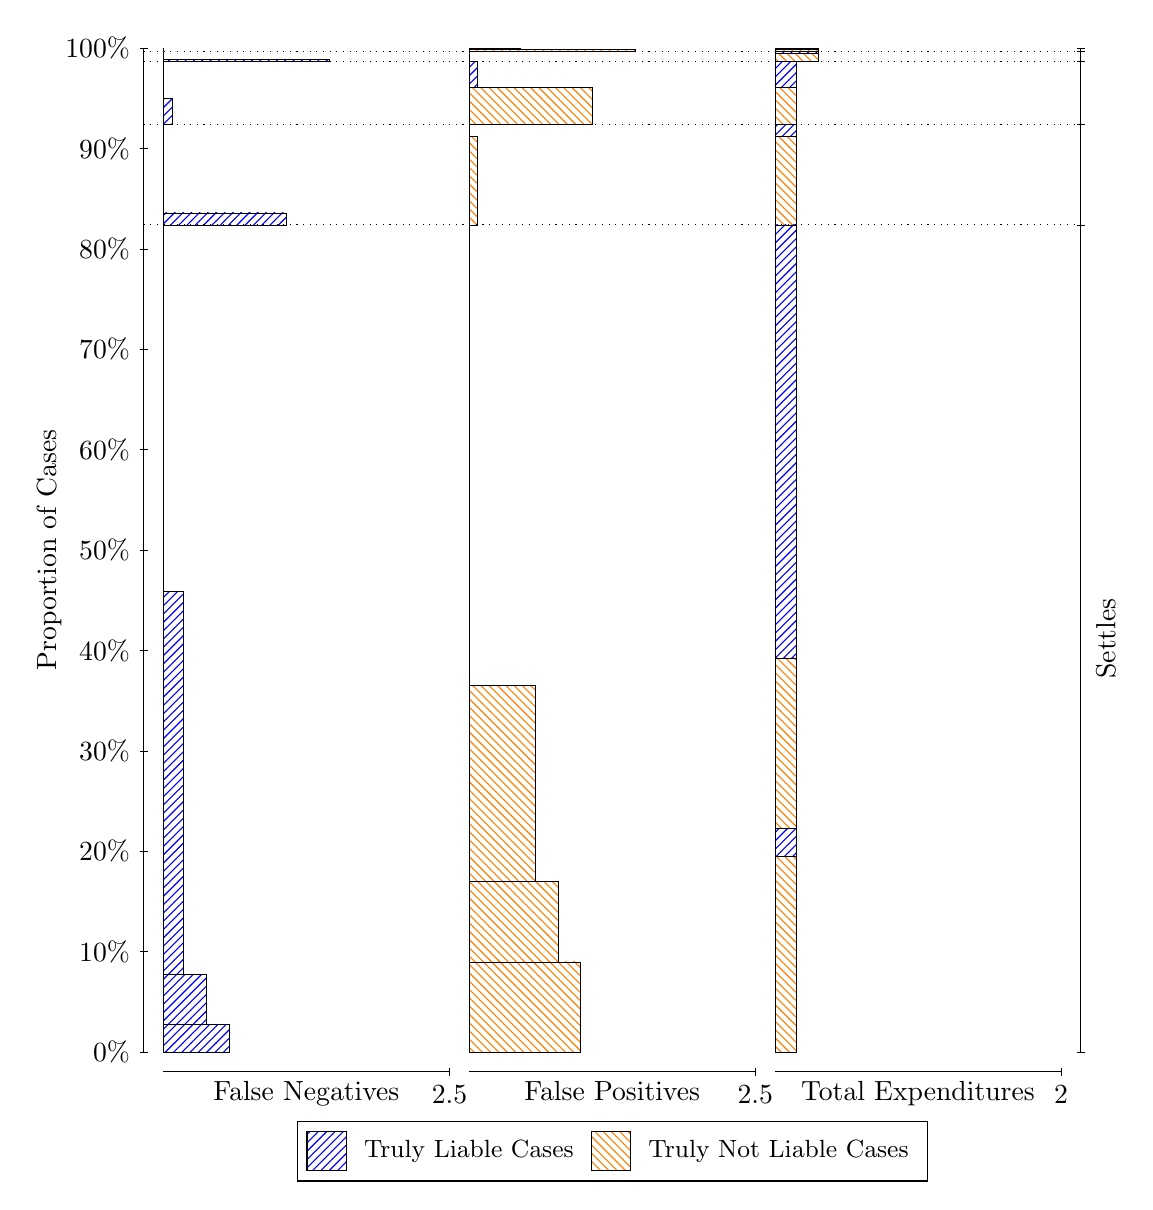
\begin{tikzpicture}
\draw[black, very thin] (1.5,1.75) -- (1.5,14.5);
\node[rotate=90, text=black, anchor=center] at (0.3, 8.125) {Proportion of Cases};
\draw[black, very thin] (1.45,1.75) -- (1.55,1.75);
\node[text=black, anchor=east] at (1.45, 1.75) {0\%};
\draw[black, very thin] (1.45,3.025) -- (1.55,3.025);
\node[text=black, anchor=east] at (1.45, 3.025) {10\%};
\draw[black, very thin] (1.45,4.3) -- (1.55,4.3);
\node[text=black, anchor=east] at (1.45, 4.3) {20\%};
\draw[black, very thin] (1.45,5.575) -- (1.55,5.575);
\node[text=black, anchor=east] at (1.45, 5.575) {30\%};
\draw[black, very thin] (1.45,6.85) -- (1.55,6.85);
\node[text=black, anchor=east] at (1.45, 6.85) {40\%};
\draw[black, very thin] (1.45,8.125) -- (1.55,8.125);
\node[text=black, anchor=east] at (1.45, 8.125) {50\%};
\draw[black, very thin] (1.45,9.4) -- (1.55,9.4);
\node[text=black, anchor=east] at (1.45, 9.4) {60\%};
\draw[black, very thin] (1.45,10.675) -- (1.55,10.675);
\node[text=black, anchor=east] at (1.45, 10.675) {70\%};
\draw[black, very thin] (1.45,11.95) -- (1.55,11.95);
\node[text=black, anchor=east] at (1.45, 11.95) {80\%};
\draw[black, very thin] (1.45,13.225) -- (1.55,13.225);
\node[text=black, anchor=east] at (1.45, 13.225) {90\%};
\draw[black, very thin] (1.45,14.5) -- (1.55,14.5);
\node[text=black, anchor=east] at (1.45, 14.5) {100\%};

\draw[black, very thin] (13.4,1.75) -- (13.4,14.5);
\draw[black, very thin] (13.35,1.75) -- (13.45,1.75);
\node[anchor=west] at (13.35, 1.75) {};
\draw[black, very thin] (13.35,12.255) -- (13.45,12.255);
\node[anchor=west] at (13.35, 12.255) {};
\draw[black, very thin] (13.35,13.534) -- (13.45,13.534);
\node[anchor=west] at (13.35, 13.534) {};
\draw[black, very thin] (13.35,14.334) -- (13.45,14.334);
\node[anchor=west] at (13.35, 14.334) {};
\draw[black, very thin] (13.35,14.457) -- (13.45,14.457);
\node[anchor=west] at (13.35, 14.457) {};
\draw[black, very thin] (13.35,14.5) -- (13.45,14.5);
\node[anchor=west] at (13.35, 14.5) {};

\draw[black, very thin, pattern color=blue, pattern=north east lines] (1.75,1.75) rectangle (2.5857,2.0988);
\draw[black, very thin, pattern color=blue, pattern=north east lines] (1.75,2.0988) rectangle (2.295,2.7335);
\draw[black, very thin, pattern color=blue, pattern=north east lines] (1.75,2.7335) rectangle (2.0043,7.5993);
\draw[black, very thin, pattern color=orange, pattern=north west lines] (1.75,7.5993) rectangle (1.75,12.255);
\draw[black, very thin, pattern color=blue, pattern=north east lines] (1.75,12.255) rectangle (3.3123,12.407);
\draw[black, very thin, pattern color=orange, pattern=north west lines] (1.75,12.407) rectangle (1.75,13.534);
\draw[black, very thin, pattern color=blue, pattern=north east lines] (1.75,13.534) rectangle (1.859,13.864);
\draw[black, very thin, pattern color=orange, pattern=north west lines] (1.75,13.864) rectangle (1.75,14.334);
\draw[black, very thin, pattern color=blue, pattern=north east lines] (1.75,14.334) rectangle (3.8573,14.358);
\draw[black, very thin, pattern color=orange, pattern=north west lines] (1.75,14.358) rectangle (1.75,14.457);
\draw[black, very thin, pattern color=orange, pattern=north west lines] (1.75,14.457) rectangle (1.75,14.48);
\draw[black, very thin, pattern color=blue, pattern=north east lines] (1.75,14.48) rectangle (1.75,14.5);
\draw[black, very thin, pattern color=orange, pattern=north west lines] (5.6333,1.75) rectangle (7.0503,2.8929);
\draw[black, very thin, pattern color=orange, pattern=north west lines] (5.6333,2.8929) rectangle (6.7597,3.9192);
\draw[black, very thin, pattern color=orange, pattern=north west lines] (5.6333,3.9192) rectangle (6.469,6.4057);
\draw[black, very thin, pattern color=blue, pattern=north east lines] (5.6333,6.4057) rectangle (5.6333,12.255);
\draw[black, very thin, pattern color=orange, pattern=north west lines] (5.6333,12.255) rectangle (5.7423,13.382);
\draw[black, very thin, pattern color=blue, pattern=north east lines] (5.6333,13.382) rectangle (5.6333,13.534);
\draw[black, very thin, pattern color=orange, pattern=north west lines] (5.6333,13.534) rectangle (7.1957,14.004);
\draw[black, very thin, pattern color=blue, pattern=north east lines] (5.6333,14.004) rectangle (5.7423,14.334);
\draw[black, very thin, pattern color=orange, pattern=north west lines] (5.6333,14.334) rectangle (5.6333,14.433);
\draw[black, very thin, pattern color=blue, pattern=north east lines] (5.6333,14.433) rectangle (5.6333,14.457);
\draw[black, very thin, pattern color=orange, pattern=north west lines] (5.6333,14.457) rectangle (7.7407,14.48);
\draw[black, very thin, pattern color=blue, pattern=north east lines] (5.6333,14.48) rectangle (6.2873,14.5);
\draw[black, very thin, pattern color=orange, pattern=north west lines] (9.5167,1.75) rectangle (9.7892,4.2365);
\draw[black, very thin, pattern color=blue, pattern=north east lines] (9.5167,4.2365) rectangle (9.7892,4.5854);
\draw[black, very thin, pattern color=orange, pattern=north west lines] (9.5167,4.5854) rectangle (9.7892,6.7545);
\draw[black, very thin, pattern color=blue, pattern=north east lines] (9.5167,6.7545) rectangle (9.7892,12.255);
\draw[black, very thin, pattern color=orange, pattern=north west lines] (9.5167,12.255) rectangle (9.7892,13.382);
\draw[black, very thin, pattern color=blue, pattern=north east lines] (9.5167,13.382) rectangle (9.7892,13.534);
\draw[black, very thin, pattern color=orange, pattern=north west lines] (9.5167,13.534) rectangle (9.7892,14.004);
\draw[black, very thin, pattern color=blue, pattern=north east lines] (9.5167,14.004) rectangle (9.7892,14.334);
\draw[black, very thin, pattern color=orange, pattern=north west lines] (9.5167,14.334) rectangle (10.062,14.433);
\draw[black, very thin, pattern color=blue, pattern=north east lines] (9.5167,14.433) rectangle (10.062,14.457);
\draw[black, very thin, pattern color=orange, pattern=north west lines] (9.5167,14.457) rectangle (10.062,14.48);
\draw[black, very thin, pattern color=blue, pattern=north east lines] (9.5167,14.48) rectangle (10.062,14.5);
\draw[black, dotted] (1.5,12.255) -- (13.4,12.255);
\draw[black, dotted] (1.5,13.534) -- (13.4,13.534);
\draw[black, dotted] (1.5,14.334) -- (13.4,14.334);
\draw[black, dotted] (1.5,14.457) -- (13.4,14.457);
\draw[black, very thin] (1.75,1.5) -- (5.3833,1.5);
\node[text=black, anchor=north] at (3.5667, 1.5) {False Negatives};
\draw[black, very thin] (5.3833,1.45) -- (5.3833,1.55);
\node[text=black, anchor=north] at (5.3833, 1.45) {2.5};

\draw[black, very thin] (5.6333,1.5) -- (9.2667,1.5);
\node[text=black, anchor=north] at (7.45, 1.5) {False Positives};
\draw[black, very thin] (9.2667,1.45) -- (9.2667,1.55);
\node[text=black, anchor=north] at (9.2667, 1.45) {2.5};

\draw[black, very thin] (9.5167,1.5) -- (13.15,1.5);
\node[text=black, anchor=north] at (11.333, 1.5) {Total Expenditures};
\draw[black, very thin] (13.15,1.45) -- (13.15,1.55);
\node[text=black, anchor=north] at (13.15, 1.45) {2};

\node[text=black, centered, rotate=90] at (13.72, 7.0025) {Settles};





\draw (7.449999999999999,1.5) node[draw=none] (baseCoordinate) {};
\begin{scope}[align=center]
        \matrix[scale=0.5, draw=black, below=0.5cm of baseCoordinate, nodes={draw}, column sep=0.1cm]{
            \node[rectangle, draw, minimum width=0.5cm, minimum height=0.5cm, pattern color=blue, pattern=north east lines] {}; &
            \node[draw=none, font=\small, text=black] (B) {Truly Liable Cases}; &
            \node[rectangle, draw, minimum width=0.5cm, minimum height=0.5cm, pattern color=orange, pattern=north west lines] {}; &
            \node[draw=none, font=\small, text=black] (B) {Truly Not Liable Cases}; \\
            };
\end{scope}

\end{tikzpicture}
\end{document}